\title{linear equations in two variables}
%\usepackage{graphicx} % Required for inserting images

\documentclass[12pt]{article}
\usepackage{amsmath}
\newcommand{\myvec}[1]{\ensuremath{\begin{pmatrix}#1\end{pmatrix}}}
\newcommand{\mydet}[1]{\ensuremath{\begin{vmatrix}#1\end{vmatrix}}}
\newcommand{\solution}{\noindent \textbf{Solution: }}
\providecommand{\brak}[1]{\ensuremath{\left(#1\right)}}
%\providecommand{\norm}[1]{\left\lVert#1\right\rVert}
\let\vec\mathbf
\usepackage{graphicx}
\graphicspath{ {./images/} }

\title{Coordinate Geometry}
\author{harshita (paidisettyharshita@sriprakashschools.com)}

\begin{document}
\maketitle
\section*{Class 10$^{th}$ Maths - Chapter 7}
This is Problem-7 from Exercise 7.4
\begin{enumerate}
\item Find the coordinates of a point A, where AB is the diameter of a circle whose centre is (2, -3) and B is (1, 4).\\
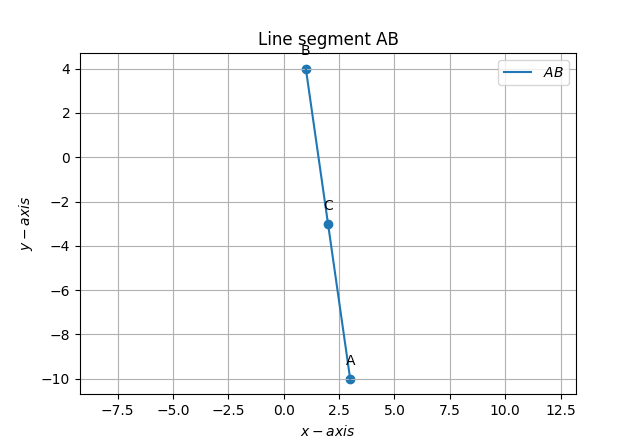
\includegraphics{/home/clab17/Figure_1.png}
\solution:
$c = \frac{mB+nA}{m+n}\\
Cm+Cn=mB+nA$\\
$\frac{Cm+Cn-mB}{n}=A$\\
\begin{align}
\vec{c} = \myvec{2\\-3}\\
\vec{b} = \myvec{1\\4} \\
\end{align}
By taking m=1 and n=1
\begin{align}
so,\\
\frac{\myvec{2\\-3}+\myvec{2\\-3}-\myvec{1\\4}}{1}
\end{align}
By adding the x,\\
2+2-1=3\\
By adding the y,\\
-3-3-4=10\\
hence,the coordinates are (3,-10)

\end{enumerate}
\end{document}